\documentclass[12pt]{article}

\usepackage{apuntes-estilo}
\usepackage{fancyhdr,lastpage}
\usepackage{color,colortbl}
\usepackage{verbatim}

\def\maketitle{

% Titulo 
 \makeatletter
 {\color{bl} \centering \huge \sc \textbf{
 Copias de seguridad (backup)\\ 
\large \vspace*{-8pt} \color{black} Guía básica de copias de seguridad (backup)
 \vspace*{8pt} }\par}
 \makeatother


% Autor
 \makeatletter
 {\centering \small 
 	Departamento de Ingeniería de Computadoras \\
 	Facultad de Informática - Universidad Nacional del Comahue \\
 	\vspace{20pt} }
 \makeatother

}

% Custom headers and footers
\fancyhf{} % clear all header and footer fields
\fancypagestyle{plain}{\fancyhf{}}
  	\pagestyle{fancy}
 	\lhead{\footnotesize Copia de seguridad - Departamento de Ingeniería de Computadoras}
 	\rhead{\footnotesize \thepage\ }	% ''Page 1 of 2''

\def\ti#1#2{\texttt{#1} & #2 \\ }



\begin{document}

\thispagestyle{empty}
\maketitle
\setlength{\parindent}{0pt}


\section*{Importancia de las copias de seguridad}
 En este apunte se explica cuándo, cómo y  por qué hacer copias de 
seguridad (backups), y de cómo recuperar información de las 
copias realizadas.

Sus datos son valiosos. Tomara tiempo y esfuerzo, si fuese necesario,
re-crearlos, y esto cuesta dinero o al menos esfuerzo extra del personal.
Algunas veces los datos no pueden ser re-creados, si por ejemplo son el 
resultado de algunos experimentos. Debido a que los datos elaborados son una 
inversión, debe protegerlos y tomar medidas para evitar pérdidas.

Existen al menos cuatro razones por la que puede perder datos: 
\begin{itemize}
\item Fallas de hardware.
\item Errores en el software. 
\item Acción humana (accidental o intencional). 
\item Desastres (incendios, inundaciones, etc). 
\end{itemize}

Si bien el hardware moderno tiende a ser confiable, puede llegar a dañarse
aparentemente de manera espontánea. La pieza más crítica para 
almacenar datos es el disco rígido, ya que se encuentra compuesto de 
pequeñísimos campos magnéticos que deben mantenerse intactos en un mundo 
lleno de interferencias electromagnéticas. Otros tipos de almacenamiento 
masivo modernos, como por ejemplo las memorias flash, si bien utilizan 
otro tipo de tecnologías, también son suceptibles de fallas.  

Por otra parte el software tiende a ser no confiable; un programa 
sólido como una roca es una excepción, no una regla. Debemos tener siempre
presente que el software está desarrollado por seres humanos y como tal, es
imperfecto. Las personas son completamente no confiables, suelen confundirse
o equivocarse, o pueden ser maliciosos y destruir los datos de forma 
intencional. Y como si esto fuera poco, existen catástrofes naturales y
humanas, como incendios, inundaciones, erupciones volcánicas, etc. 
que pueden causar estragos en lo referente a pérdida de datos.  

\fcolorbox{black}{grey}{
\parbox[t]{1.0\linewidth}{ \vspace*{0.4cm}
{\bf En resumen}: en computación, es un pequeño milagro que las cosas 
funcionen bien y sin interrupción. Por lo que, es imperioso tomar medidas
 para minimizar las pérdidas de datos y los costos asociados a las mismas. 
\vspace*{0.4cm} } }

Las copias de seguridad son una manera de proteger la inversión realizada 
en los datos. Las pérdidas de información tienen menor impacto si existen 
varias copias resguardadas, en tal caso existirá solo el costo que conlleve
recuperar los datos perdidos desde las copias, que en muchos casos, 
dependiendo de la criticidad de la información puede ser   
considerable. 

Es importante realizar copias de seguridad correctamente. Como todo lo 
relacionado con el mundo físico, se dañarán tarde o temprano. Parte del
trabajo al realizar copias de seguridad es estar seguro de que estas 
funcionan; ya que no desea enterarse tiempo después que las copias no son 
útiles.\footnote{No reírse. Esto le sucede a muchas personas.} Además,
 piense en estos dos casos: sus datos podrían dañarse justo en el momento 
en que esta realizando copias de seguridad; o, si solamente tiene un medio 
para copias de seguridad, podría llegar a romperse también. 

O se entera, cuando intenta recuperar, que olvidó respaldar algo importante,
como la base de datos de los usuarios en un sitio con miles de usuarios. 
Finalmente, el mejor de todos los casos: las copias de seguridad trabajan 
perfectamente, pero la última unidad sobre la faz de la Tierra que lee el 
tipo de cinta que usted utilizaba, está llena de agua y se ha dañado 
irreparablemente.

Cuando de copias de seguridad se trata, la paranoia está en la descripción 
de la tarea.

\section*{Seleccionando el medio de backup}

La decisión mas importante al pensar en hacer copias de seguridad es la 
selección del medio a utilizar. Necesita considerar el costo, 
confiabilidad, velocidad, disponibilidad y usabilidad.

El \texttt{costo} es importante, porque preferentemente desea contar con 
mayor 
capacidad de almacenamiento para los backups de lo que necesita para los 
datos existentes. Un medio económico es usualmente casi una obligación.

La \texttt{confiabilidad} es una característica de extrema importancia, 
ya que una 
copia de seguridad dañada puede hacer llorar a un gigante. Un medio para 
copias de seguridad debe ser capaz de mantener los datos en perfecto 
estado durante años. Además, la forma en que se utiliza el medio afecta 
a su confiabilidad. Un disco rígido es típicamente muy confiable, pero 
no como medio para copias de seguridad en caso de que se encuentre en 
la misma computadora en donde están los discos al que se les realiza la 
copia.

La \texttt{velocidad} usualmente no muy importante, en caso de que la 
copia pueda ser
realizada sin interacción. No importa que el backup demore unas 
dos horas, o lo que fuese necesario si no necesita atención. En cambio, si 
la copia no puede ser realizada cuando la computadora se encuentre ociosa, 
considere a la velocidad del medio al momento de la elección.

La \texttt{disponibilidad} es obviamente necesaria, debido a que no se 
puede utilizar
un medio para copias de seguridad si no existe. Menos obvio es la 
disponibilidad futura, y en otras computadoras diferentes a las que se 
utilizaron para generar las copias.
Si este caso sucede, puede no ser posible realizar una recuperación de la 
información luego de un desastre.

Las alternativas típicas son los discos ópticos (CD, DVD, BluRay) y las
cintas. Los discos ópticos son baratos, relativamente confiables, no muy 
rápidos, muy disponibles, pero no muy útiles para grandes cantidades de 
información (Blu-ray almacena alrededor de 25G de datos). Las 
cintas varían en cuanto a su valor, generalmente son baratas aunque algunos
tipos no lo son tanto, relativamente confiables y veloces, muy disponibles, 
y generalmente (aunque depende de su capacidad) son útiles para almacenar 
mucha información (en el orden de los cientos de giga a tera byte). 


\begin{figure}[h]
\centering
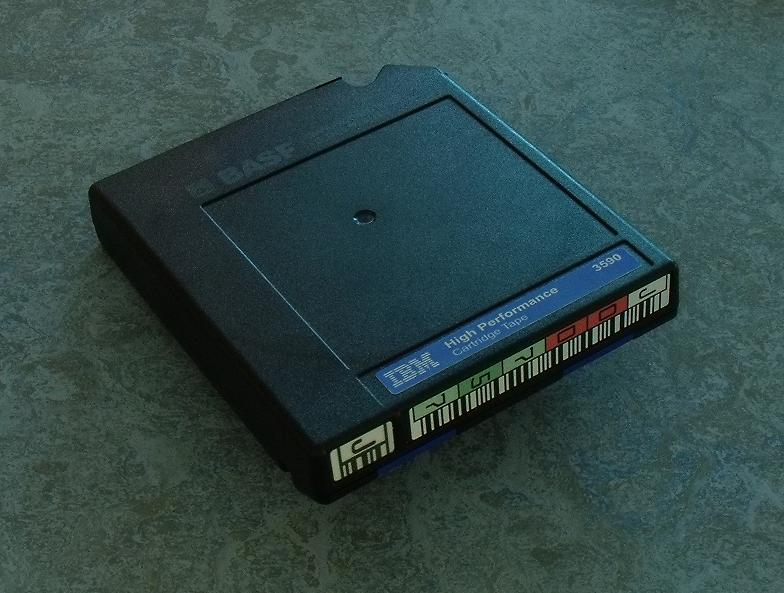
\includegraphics[width=0.8\textwidth]{3590Tape.JPG}
\renewcommand{\figurename}{Fig.}
\caption{IBM 3590 data cartridge almacena hasta 10GiB sin compresión}
\label{contexto:figura}
\end{figure}

Para copias de seguridad de datos de computadora y transferencia de datos 
física, los discos ópticos como el CD y el DVD están siendo reemplazados 
gradualmente por dispositivos de estado sólido más rápidos, pequeños y 
confiables, especialmente la memoria USB. Se espera que esta tendencia 
continúe a medida que las memorias USB sigan creciendo en capacidad y 
disminuyendo sus precios. 
	
\section*{Seleccionando la herramienta de backup}

Existen muchas herramientas que pueden ser utilizadas para realizar las 
copias de seguridad.  Las herramientas tradicionales en entornos UNIX 
son \texttt{\textbf{tar}}, \texttt{\textbf{cpio}} y \texttt{\textbf{dump (que incluye los comandos 
dump y restore)}}.
 Además, existe un gran 
número de software de terceros (comerciales y libres como
 Amanda\footnote{http://www.amanda.org/}) que pueden ser 
utilizados. La selección del medio para copias de seguridad puede afectar 
a la selección de la herramienta a utilizar.

Los comandos \texttt{\textbf{tar}} y \texttt{\textbf{cpio}}
son similares, y casi completamente equivalentes desde el punto de 
vista de los backups. Ambas son capaces de almacenar y recuperar 
archivos en cintas. También son capaces de utilizar 
prácticamente cualquier medio, debido a que los controladores de 
dispositivos del kernel son los que se encargan del acceso al hardware a 
bajo nivel; por lo que todos los dispositivos
tienden a verse de la misma manera para los programas en espacio de usuario.
Algunas versiones  UNIX antiguas de \texttt{\textbf{tar}} y 
\texttt{\textbf{cpio}} pueden tener dificultades con archivos inusuales 
(enlaces simbólicos, archivos de dispositivos, archivos con nombres
muy largos, etc.), pero las versiones GNU/Linux de estas herramientas 
deberían manejar toda clase de archivos correctamente.

El comando \texttt{\textbf{dump/restore}} es diferente a las dos herramientas 
anteriores, debido a que lee el sistema de archivos directamente, y no a 
través del sistema de archivos.  Además, fue desarrollado específicamente 
para generar copias de seguridad; \texttt{\textbf{tar}} y 
\texttt{\textbf{cpio}} son empaquetadores de archivos 
(a pesar de que también trabajan como herramientas para backups).

Leer el sistema de archivos directamente tiene algunas ventajas.
Si es necesario copiar todo el sistema de archivos, entonces la lectura 
directa es mas efectiva, debido a que se realizan muchos menos movimientos 
de la cabeza lecto-escritora del disco. La mayor desventaja es que dump es 
un programa de copia específico para solamente un tipo de sistemas de 
archivos; el programa \texttt{\textbf{dump/restore}} de GNU/Linux puede leer 
únicamente los sistema de archivos ext2/3/4. Al ser diseñado para copias
de seguridad, \texttt{\textbf{dump}} soporta distintos niveles de copias
 (tema que se encuentra explicado en páginas posteriores); con 
\texttt{\textbf{tar}} y \texttt{\textbf{cpio}} los niveles de copia de 
seguridad debe ser implementado utilizando otras herramientas.

Una comparación con herramientas de terceros para copias de seguridad se 
encuentra fuera del alcance de este apunte. Existen diversas soluciones, 
cada una se adapta a una necesidad particular y deberán ser evaluadas 
cuando las herramientas presentadas no respondan a las necesidades. 

\section*{Modelos de copias de seguridad}
Desde los primeros años de uso de copias de seguridad, se han desarrollado 
nuevas tecnologías que han intentado minimizar en la medida de lo posible 
el tamaño de los datos almacenados, el tiempo de copia y el tiempo de 
restauración de los mismos.

Fruto de estas investigaciones son los tres modelos básicos que hoy 
día se utilizan en los procesos de generación de copias de seguridad:
\begin{itemize}
\item Copia total o completa (full backup).
\item Copia diferencial.
\item Copia incremental.
\end{itemize}

La decisión de cuál de los métodos anteriormente citados se ha de 
utilizar cambia con las circunstancias particulares de cada situación 
y en la mayoría de los casos depende fundamentalmente de cuatro factores:

\begin{itemize}
\item La capacidad de los soportes sobre los que se va a grabar la 
información.
\item El período de tiempo disponible para hacer la copia.
\item El medio en el que se desarrolla el trabajo (local, intranet, 
internet, etc.).
\item El nivel de urgencia a la hora de necesitar restaurar los datos.
\end{itemize}

Independientemente de los factores que determinen el tipo de copia a 
realizar, en la práctica, una buena política de gestión de copias de 
seguridad incluirá la conjunción de varios de los modelos expuestos. Una 
buena política de cooperación entre modelos de copias de seguridad 
garantizará un buen resultado final y la obtención de un seguridad
de datos fiable, robusto y rápido.

\subsection*{Copia total o completa}
Es el tipo básico e ideal de copia de seguridad ya que es el más 
exhaustivo y autónomo, y en el que se basan el resto de modalidades.

Una copia total incluye todos y cada uno de los archivos seleccionados
para ser incluidos en el proceso de copia, sin importar si han 
sufrido cambio o no desde la última vez que se realizó la copia anterior.

Es la forma de copia de seguridad de más tiempo y recursos (léase espacio 
de almacenamiento) consume, pero la más rápida y segura a la hora de 
recuperar datos de ella. 

\subsection*{Copia diferencial}
La copia diferencial supone la existencia de una copia total existente, y
contiene todos los archivos que han cambiado desde la última
copia completa. Las copias diferenciales son acumulativas entre sí, es 
decir, si se tienen programadas varias copias diferenciales entre copias
 totales, cada una de ellas no tendrá en cuenta la anterior e irá 
acumulando los cambios desde la última total.


\begin{figure}[h]
\centering
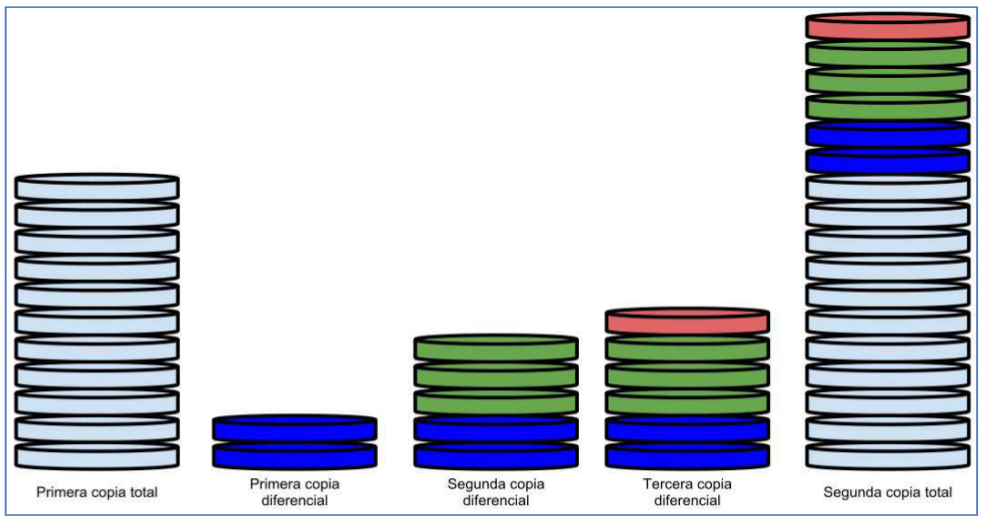
\includegraphics[width=0.8\textwidth]{diferencial.png}
\renewcommand{\figurename}{Fig.}
\caption{Copia diferencial}
\label{contexto:figura}
\end{figure}

\subsection*{Copia Incremental}
Las copias de tipo incremental contienen únicamente los archivos que fueron
modificados o creados desde la última copia total, o incremental. La 
diferencia fundamental respecto a las copias diferenciales, es que no son 
redundantes (la información no se repite de una copia a la siguiente).


\begin{figure}[h]
\centering
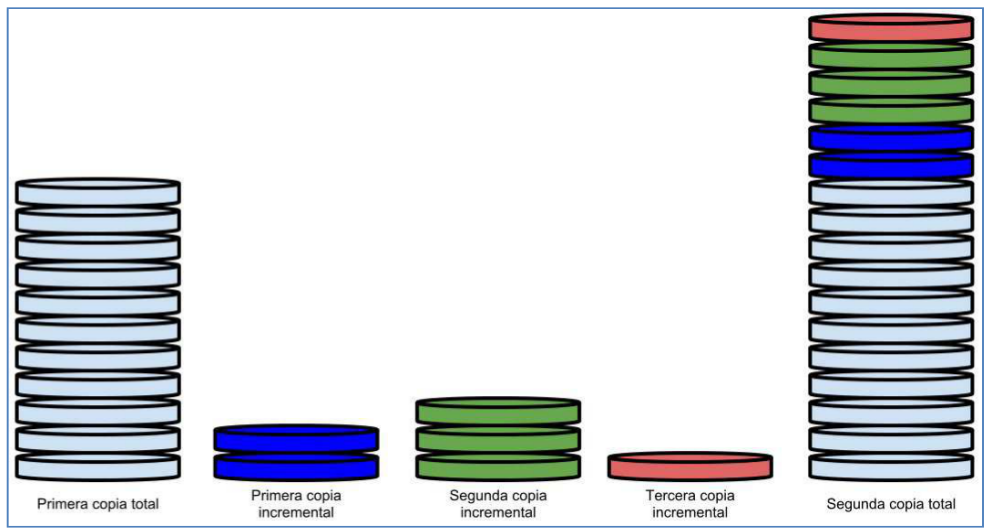
\includegraphics[width=0.8\textwidth]{incremental.png}
\renewcommand{\figurename}{Fig.}
\caption{Copia incremental}
\label{contexto:figura}
\end{figure}

\subsection*{Un esquema sencillo}

Un esquema simple de copias de seguridad es respaldar todo una única vez, 
y luego, copiar solamente los archivos que fueron modificados después de 
la copia inicial. La primera copia se denomina \textit{copia total (full 
backup)}, y las siguientes son \textit{copias incrementales 
(incremental backups)}. Una copia total frecuentemente necesita de mayor 
esfuerzo para ser generada, debido a que hay mas datos a escribir,
y eventualmente (o frecuentemente) puede no caber en una única cinta, o 
cualquiera que sea el medio utilizado.
De manera opuesta, recuperar información desde las copias
incrementales necesita muchas veces mas empeño que hacerlo desde una copia 
total. La recuperación puede ser optimizada si cada copia incremental se 
realiza con respecto a la copia total previa. De esta manera, las copias 
pueden necesitar un poquito mas de esfuerzo (y demorar mas también), 
pero nunca será necesario recuperar mas que dos copias (una total y una 
incremental).

El siguiente es un ejemplo simplificado basado en cintas, lo mismo podría 
pensarse utilizando otros medios. 
En caso de que desee realizar copias todos los días y tenga seis cintas, 
puede utilizar la cinta 1 para la primera copia completa (digamos, un 
viernes), y utiliza las cintas 2 a 5 para las copias incrementales 
(lunes a jueves). El segundo viernes, realiza una nueva copia total en la 
cinta 6, y reinicia nuevamente el ciclo de copias incrementales con las 
cintas 2 a 5. No es conveniente sobreescribir la cinta 1 hasta que una 
nueva copia completa haya sido generada. Después del segundo viernes, debe
mantener la cinta 1 en un lugar físico distinto del resto. De esta manera, 
si el conjunto de cintas 2 a 6 se dañan en un incendio, tiene al menos una 
copia completa en un lugar seguro (esta copia tiene una semana de 
antigüedad, pero es mejor que nada).  Cuando necesite realizar la próxima 
copia total, utilice la cinta 1 y coloque la cinta 6 el el lugar seguro.

En caso de que disponga con mas de 6 cintas, puede utilizar las cintas 
extras para las copias completas. Y cada vez que realice una copia total 
utilizará la cinta mas antigua. De esta manera puede almacenar copias
completas de varias semanas previas, lo cual es útil en caso de que necesite
encontrar un archivo que ha sido borrado, o desea recuperar una vieja 
versión de algún otro.

\section*{Utilizando \texttt{tar}}
GNU tar crea y manipula archivos que en realidad son colecciones de muchos 
otros archivos, el programa proporciona a los usuarios un método organizado 
y sistemático para controlar una gran cantidad de datos. El nombre de 
``tar'' vino originalmente de la frase ``Tape ARchive'' (archivo en cinta),
pero los archivos no necesitan (y en estos días, por lo general no lo hacen)residir en las cintas.


Puede utilizar los archivos de tar de muchas maneras. Queremos destacar 
algunos de ellos: el almacenamiento, copia de seguridad y transporte.

{\bf Almacenamiento y transporte:}

A menudo, los archivos tar se utilizan para almacenar los archivos 
relacionados para una cómoda transferencia de archivos a través de una red.
Por ejemplo, el proyecto GNU distribuye su software incluido con los 
archivos tar, por lo que todos los archivos relacionados con un determinado 
programa (o conjunto de programas relacionados) se pueden transferir como 
una sola unidad.

Una cinta magnética puede almacenar varios archivos en secuencia. Sin
 embargo, la cinta no tiene nombres para estos archivos, sino que sólo 
conoce su posición relativa en la cinta. Una forma de almacenar varios 
archivos en una cinta y retener sus nombres es mediante la creación de un 
archivo tar. 

{\bf Copia de seguridad}

Debido a que el archivo creado por el tar es capaz de conservar la 
información del archivo y la estructura de directorios, tar se utiliza 
habitualmente para realizar copias de seguridad completas e incrementales 
de discos. GNU tar tiene características especiales que le permiten ser
utilizado para hacer volcados incrementales y completos de todos los 
archivos en un sistema de archivos.

\subsection*{Realizando copias de seguridad}
Una copia completa puede realizarse fácilmente con \texttt{\textbf{tar}}:

\fcolorbox{black}{grey}{
\parbox[t]{1.0\linewidth}{ \vspace*{0.4cm}
{\tt
\# tar --create --file /dev/st0 /home \\
}
El dispositivo {\tt /dev/st0} representa a la primer cinta magnética del
sistema. El comando anterior creará un backup del directorio /home en dicha
cinta.  
\vspace*{0.4cm} } }

El ejemplo anterior utiliza la versión GNU de \texttt{\textbf{tar}} y sus 
nombres de opciones largos a modo explicativo. Normalmente utilizaremos 
\texttt{\textbf{tar}} con opciones de un único caracter. Por ejemplo el 
comando anterior es equivalente a {\tt tar -cf /dev/st0 /home}. 
Además, la versión GNU puede manejar copias que no quepan completamente 
en una cinta (o medio utilizado), y con caminos de
directorios muy largos; no todas las versiones de tar pueden hacer eso. 
(GNU/Linux solo utiliza GNU \texttt{\textbf{tar}}.)  

En caso de que la copia no quepa en una única cinta, es necesario activar la
 opción ``{\tt --multi-volume}'' o ``{\tt -M}''. 

Después de realizar una copia, debe verificar si todo se encuentra en 
correctas condiciones utilizando la opción ``{\tt --compare}, ``{\tt -d} ó 
``{\tt --diff}. 

\colorbox{grey}{\parbox[t]{0.95\linewidth}{ \vspace*{0.5cm} { 
{\bf Ejemplo:} en la siguiente secuencia se ve el uso de la opción ``-d'',
y como el comando \texttt{tar} reporta una diferencia luego de eliminar 
un archivo.\\ 
{\tt
\$ tar -cf tsl.tar TSL/\\
\$ tar -df tsl.tar TSL/\\
\$ cd TSL/\\
\$ ls\\
AdminSis2013  gasl-ac  Primer\_Parcial\_Admin\_2013.ods\\
\$ cd AdminSis2013/\\
\$ ls\\
BD\_alumnos\_2013\_Admin\_-22\_records-20130824\_2341-comma\_separated.csv\\
BD\_alumnos\_2013\_Admin\_-27\_records-20130910\_1426-comma\_separated.csv\\
BD\_alumnos\_2013\_Admin\_-29\_records-20130914\_2109-comma\_separated.csv\\
examen1\\
ProgramaAdministraciónSistemas.odt\\
ProgramaAdministraciónSistemas.pdf\\
Turnos\_1er\_parcial.pdf\\
\$ rm Turnos\_1er\_parcial.pdf \\
\$ cd \\
\$ tar -df tsl.tar TSL/\\
tar: TSL/AdminSis2013/Turnos\_1er\_parcial.pdf: Atención: No se puede stat:
No existe el fichero o el directorio\\
}
Nótese que en este ejemplo sólo se está creando un  archivo {\tt tsl.tar} 
en el mismo sistema de archivos que el original. Para que efectivamente 
este archivo constituya una copia de seguridad sería prudente guardarlo 
en otro medio de almacenamiento. 
} \vspace*{0.5cm} } } 

El comando {\tt tar} posee muchas opciones para seleccionar un subconjunto
de archivos, por ejemplo la opción ``{\tt --newer}'' o ``{\tt -N} nos 
permite archivar sólo archivos creados luego de una cierta fecha.  

\subsection*{Recuperando archivos }

Para recuperar archivos desde una copia de seguridad creada con {\tt tar} se
debe utilizar la opción ``{\tt --extract}'' o, su forma corta ``{\tt -x}''. 

\colorbox{grey}{\parbox[t]{0.95\linewidth}{ \vspace*{0.5cm} { 
{\bf Ejemplo:} restaurando archivos desde una cinta magnética. \\
{\tt
\#tar --extract --same-permissions --verbose --file /dev/st0\\
usr/src/\\
usr/src/linux\\
usr/src/linux-1.2.10-includes/\\
usr/src/linux-1.2.10-includes/include/\\
usr/src/linux-1.2.10-includes/include/linux/\\
usr/src/linux-1.2.10-includes/include/linux/hdreg.h\\
usr/src/linux-1.2.10-includes/include/linux/kernel.h\\
\#\\
}
} \vspace*{0.5cm} } } 

También puede extraer archivos y directorios específicos (los cuales 
incluyen todos sus archivos y subdirectorios). Basta con mencionarlos en 
la línea de comandos:

\colorbox{grey}{\parbox[t]{0.95\linewidth}{ \vspace*{0.5cm} { 
{\bf Ejemplo:} continuando con el ejemplo del archivado en el archivo 
{\tt tsl.tar}, vemos como recuperar desde la copia de seguridad un archivo
que fue eliminado por error: \\
{\tt
\$ rm TSL/Primer\_Parcial\_Admin\_2013.ods \\
\$ tar xvf tsl.tar TSL/Primer\_Parcial\_Admin\_2013.ods \\
\\TSL/Primer\_Parcial\_Admin\_2013.ods\\
\$ ls -l TSL/Primer\_Parcial\_Admin\_2013.ods\\
\-rw-r--r-- 1 lechnerm lechnerm 21804 sep 16 08:04 TSL/Primer\_Parcial\_Admin\_2013.ods\\
\$ \\
}
} \vspace*{0.5cm} } } 

Utilice la opción ``{\tt --list}'' (o su forma corta ``{\tt -t}'') para 
es son los archivos presentes en un volumen de backup, sin efectivamente 
extraerlos del mismo:

\colorbox{grey}{\parbox[t]{0.95\linewidth}{ \vspace*{0.5cm} { 
{\bf Ejemplo:} continuando con el contenido de la cinta magnética, el 
siguiente comando listará pero no extraerá los datos de la cinta.\\  
{\tt
\#tar --list --file /dev/st0\\
usr/src/\\
usr/src/linux\\
usr/src/linux-1.2.10-includes/\\
usr/src/linux-1.2.10-includes/include/\\
usr/src/linux-1.2.10-includes/include/linux/\\
usr/src/linux-1.2.10-includes/include/linux/hdreg.h\\
usr/src/linux-1.2.10-includes/include/linux/kernel.h\\
\#\\
}
} \vspace*{0.5cm} } } 

Note que \texttt{\textbf{tar}} siempre lee el volumen de la copia de 
seguridad secuencialmente, lo que puede llegar a ser lento para grandes 
volúmenes.  De cualquier manera, si utiliza medios secuenciales como 
cintas, no es posible el acceso aleatorio.

\subsection*{Copia completa}
{\bf Las copias completas sólo deben realizarse cuando no hay personas o 
programas que están modificando los archivos del sistema de archivos}. Si 
los archivos se modifican mientras tar está haciendo la copia de seguridad,
no pueden ser almacenados adecuadamente en el archivo tar de salida, en 
cuyo caso no podrá restaurarlos si es necesario. (Los archivos que  no 
están siendo modificados se escriben sin ningún problema, y no corrompen 
todo el archivo.)

A menos que el sistema de archivos que se está volcando quepa en un solo 
volumen, tendrá que utilizar la opción ``{\tt --multi-volume}'' 
(``{\tt -D}'') para varios volúmenes.  Asegúrese de tener suficientes 
cintas (u otro medio) a mano para completar la copia de seguridad.

Considerando que pueden existir múltiples sistemas de archivos montado a lo
largo de la jerarquía de directorios, si se desea crear copias de seguridad,
de cada sistema de archivos por separado, se deberá utilizar la opción 
``{\tt --one-file-system}'' para evitar que tar cruce los límites
del sistema de archivos al guardar (sub) directorios.

A menos que se esté apurado, y confíe en el programa tar (y sus cintas),
es una buena idea utilizar la opción ``{\tt --verify}'' (``{\tt -W}''),
para asegurarse de que sus archivos se encuentran efectivamente en la 
copia de respaldo. Esto también ayuda a detectar los casos en que se 
modificó el archivo mientras (o inmediatamente después) que estaba siendo
archivado. No todos los medios de comunicación (en particular, las cintas 
de cartucho) son capaces de ser verificado, por desgracia.

\subsection*{Copia incremental}
Una copia de seguridad incremental es una forma especial de archivo tar que 
almacena metadatos adicionales para que el estado exacto del sistema de 
archivos se pueden restaurar cuando se extrae el archivo.

GNU tar actualmente ofrece dos opciones para el manejo de copias de 
seguridad incrementales: ``{\tt --listed-incremental=snapshot-file}'' 
(``{\tt -g snapshot-g-file}'') e ``{\tt --incremental (-G )}''.

La opción ``{\tt --listed-incremental }'' indica a tar operar en un archivo 
incremental con metadatos adicionales almacenados en un archivo 
independiente, denominado \textit{archivo de instantánea} (en inglés, 
snapshot file). La finalidad de este fichero es la de ayudar a determinar 
qué archivos se han cambiado, añadido o eliminado desde la última copia 
de seguridad, de modo que la siguiente copia de seguridad incremental 
contendrá sólo los archivos modificados. El nombre del archivo de 
instantánea se da como argumento para la opción:


\colorbox{grey}{\parbox[t]{0.95\linewidth}{ \vspace*{0.5cm} { 
{\bf Ejemplo: usando --listed-incremental } \\
{\tt
\# tar --create \textbackslash \\
           --file=archive.1.tar \textbackslash \\
           --listed-incremental=/var/log/usr.snar \textbackslash \\
           /usr \\
}
Esto creará en {\tt archive.1.tar} una copia de seguridad incremental del 
sistema de archivos {\tt /usr}, y almacenará metadatos adicionales en el 
archivo {\tt /var/log/usr.snar}. Si este archivo no existe, se creará.
} \vspace*{0.5cm} } } 

El archivo creado en el ejemplo será una copia de seguridad de nivel cero, 
copia completa la primera vez que lo realizamos. Luego, si el archivo
{\tt /var/log/usr.snar} existe, tar determinará cuáles de los archivos 
listados fueron modificados. En cuyo caso, sólo estos últimos serán 
almacenados en el archivo. 

Luego de creado esta primera copia, podemos hacer una copia de seguridad
incremental de nivel uno utilizando el archivo instantánea: 


\colorbox{grey}{\parbox[t]{0.95\linewidth}{ \vspace*{0.5cm} { 
{\bf Ejemplo: usando --listed-incremental para copia de nivel uno } \\
Asumiendo que se han cambiado algunos archivos desde la copia de nivel 
cero, creamos una copia de nivel uno incremental: \\
{\tt
\# cp /var/log/usr.snar /var/log/usr.snar-1 	\\
\# tar --create \\\
           --file=archive.2.tar \textbackslash \\
           --listed-incremental=/var/log/usr.snar-1 \textbackslash \\
           /usr\\
tar: usr/local/db: Directory is new\\
usr/local/db/\\
usr/local/db/data\\
usr/local/db/index\\
}
Nótese que copiamos el archivo de instantánea antes de crear una nueva 
copia de seguridad, dado que podríamos querer crear más de una copia 
de nivel uno a partir de la primera copia de nivel cero. Si utilizáramos 
el mismo archivo, este se actualizaría a partir de la última copia 
incremental. 
} \vspace*{0.5cm} } } 



\section*{Copias de seguridad comprimidas}

Las copias de seguridad ocupan una gran cantidad de espacio, por lo que
puede ser costoso al momento de invertir en el medio a utilizar.
Para reducir el espacio necesario la copias de seguridad pueden ser 
comprimidas.  Existen varias formas de hacerlo, pero una de la mas práctica 
es utilizar directamente programas con soporte para compresión.

Por ejemplo GNU \texttt{\textbf{tar}}, cuya opción ``{\tt --gzip}'' o 
``{-z}'' hace que la información resguardada sea procesada por el programa 
de compresión \texttt{\textbf{gzip}} antes de ser copiada al medio para 
backups.
	
Desafortunadamente las copias de seguridad comprimidas pueden causar 
problemas. Debido a la naturaleza de como la compresión funciona, si un 
simple bit es incorrecto, todo el resto de los datos comprimidos son 
inutilizables. Algunos programas para backups pueden corregir algunos de 
estos errores, pero ningún método de los implementados 
pueden manejar un gran número de errores. Esto significa que si la copia de 
seguridad es comprimida en la manera en que GNU \texttt{\textbf{tar}} lo 
hace (la salida de la copia comprimida es una única unidad), el backup 
completo puede ser inútil si tan solo existe un simple error.

Las copias deben ser confiables, y este método de compresión no es una 
buena idea. Una manera alternativa es comprimir cada uno de los archivos 
separadamente. El problema mencionado anteriormente aún persiste, pero si 
un archivo en el backup se encuentra dañado, al menos los demás no sufren 
los efectos colaterales. También se debe tener en cuenta que no todos los 
datos son susceptibles de ser comprimidos; mientras que un archivo de 
texto reduce considerablemente su tamaño al ser comprimido por gzip, un
archivo de imagen puede diferir en muy poco de su versión original a menos
que se utilice software de compresión de imágenes especifico. 

Por otro lado, la compresión lleva también lleva tiempo y alto consumo 
de CPU, por ello y por lo expuesto en los párrafos anteriores, es importante
hacer un análisis profundo de la necesidad o no de aplicar compresión.
	
\section*{Qué copiar}

Establecer con claridad cuál es la información a respaldar es una tarea 
compleja que requiere un profundo conocimiento del entorno de trabajo. 
Usualmente requerirá de un análisis de las políticas de almacenamiento 
de datos de la empresa y de las conductas propias de los usuarios, acotado
por los medios y sistemas de copia de seguridad disponibles.  

Es necesario crear un inventario (existe software dedicado a este fin), que
permita listar todos los equipos de la empresa y sus características de 
configuración mínimas, como ser: cantidad de discos conectados, tabla de
particiones de cada disco e información de manejador de volúmenes si los 
hubiera, función del equipo, tipo de hardware, listado de sistema de 
archivos, etc. El inventario nos permite tener una visión de la magnitud
del esfuerzo necesario para establecer copias de seguridad, así como 
también determinar y priorizar las tareas de recuperación ante un eventual
desastre. 

En principio uno debe respaldar la mayor cantidad de información posible, 
tal que ante una eventual pérdida de datos, permita restituir los mismos 
con la celeridad necesaria para minimizar las pérdidas económicas y 
continuar con la operación del negocio. 

La mayor excepción en general es el software (aunque pueden existir 
excepciones), ya que puede ser fácilmente reinstalado. Aunque la 
re-instalación puede tomar tiempo, por lo que la velocidad de recuperación
es un factor a considerar. 
Tenga en cuenta que los programas muchas veces están configurados 
manualmente para sus sistemas, por lo que es importante respaldar a los 
archivos de configuración, y evitar así la tarea de reconfigurarlos 
nuevamente. En el caso particular de GNU/Linux, hacer una copia de
seguridad del directorio {\tt /etc/} es imperioso en este sentido.

Otra gran excepción son los sistemas de archivos temporales, creados por 
el sistema operativo durante su ejecución, como ser el montado en 
\texttt{/proc}, debido a que solamente contiene información que el kernel
genera automáticamente. Por lo que nunca es buena idea copiarlo, 
especialmente el archivo \texttt{/proc/kcore} es innecesario, ya que 
solamente es una imagen de la memoria física, y nunca suele ser muy útil 
dentro de un backup (solo ocupa bastante espacio).
	
Hay algunas otras partes de un sistema GNU/Linux que deben ser analizadas
 antes de ser incluidas en sus copias de seguridad. Por ej., los archivos 
de log, las colas de los archivos de impresión, las news y muchas otras 
cosas que se encuentran bajo \texttt{/var}. 

Debe decidir que considera importante y que no.  Lo obvio al momento de 
respaldar son los archivos de los usuarios (\texttt{/home}) y los archivos
de configuración del sistema (\texttt{/etc}, y posiblemente otros archivos
y directorios que se encuentren dispersos en el sistema de archivos que, 
por ejemplo contengan información producida por el uso de las aplicaciones
del sistema.



\section*{Referencias}

GNU/tar: http://www.gnu.org/software/tar/manual/

``Trabajo final de carrera: Copias de seguridad - Estudio y metodología''.
Rafael Santamaría Carmona. Universitat Oberta de Catalunya.

\section*{Licencia}
This is a derived version of "Guía Para Administradores de Sistemas GNU/Linux" that 
can be found at \\ \texttt{http://www.ibiblio.org/pub/Linux/docs/LDP/system-admin-guide/translations/es/gasl.txt}.

Copyright (C) 1993-1998 Lars Wirzenius.

Copyright (C) 1998-2001 Joanna Oja.

Copyright (C) 2001-2003 Stephen Stafford.

Copyright (C) 2003-2004 Stephen Stafford and Alex Weeks.

Copyright (C) 2004-Present Alex Weeks.

Copyright (C) 2013-Present Rafael Ignacio Zurita

Trademarks are owned by their owners.

Permission is granted to copy, distribute and/or modify this document under
the terms of the GNU Free Documentation License, Version 1.2 or any later
version published by the Free Software Foundation; with no Invariant
Sections, no Front-Cover Texts, and no Back-Cover Texts. A copy of the
license is included in the section entitled "GNU Free Documentation License".

\subsection*{Traducción de la licencia}
Esta es una obra derivada de "Guía Para Administradores de Sistemas GNU/Linux" que puede 
econtrarse en \\ \texttt{http://www.ibiblio.org/pub/Linux/docs/LDP/system-admin-guide/translations/es/gasl.txt}.

Las marcas registradas son propiedad de sus dueños.

Se concede autorización para copiar, distribuir y/o modificar este documento
bajo los términos de la Licencia de documentación libre GNU (FDL), Versión 1.2; 
sin Secciones Invariantes, sin textos de Portada, y sin Textos de Contra Portada. 
Una copia de la licencia se encuentra incluída en la sección "GNU Free Documentation License".


\end{document}
